\chapter{Multi-Echo Radial FLASH} \label{Chp:multi-echo}
\chaptermark{Multi-Echo Radial FLASH}

%The conventional \textit{multi-echo} radial FLASH utilizes bipolar readout gradients with the same amplitude and duration to sample echoes in a fly-back-and-forth manner, which, however, is not efficient enough in the respects of k-space coverage and temporal resolution. Therefore, the multi-echo multi-spoke radial FLASH sequence, which acquires multiple echoes with different spatial encodings per RF excitation, is proposed for the purposes of faster k-space sampling and better temporal resolution. In addition, a nonlinear inverse reconstruction that jointly estimates all echo images and coil sensitivity maps is investigated.
%In this chapter, two types of multi-echo radial FLASH sequences with preliminary results including phantom, human brain and cardiac studies are presented. 

\section{Introduction}
Multi-gradient-echo sequences contain two intrinsic properties. First, they acquire multiple echoes after one RF excitation, which substantially shortens imaging time when echoes are differently encoded. Note that one TR interval in these sequences is also named one echo-train. Second, they elongate TE and TR, resulting in \acs{T2s}-weighted image contrast and off-resonance phase modulations among echoes. $T_2^*$ signal decay is a direct indication of the blood-oxygen-level dependent (\acs{BOLD}) contrast primarily used in functional MRI (\acs{fMRI}), discovered by Ogawa et al.~in 1990 \cite{1990_fMRI}. Nowadays, the most frequently used sequence for fMRI is echo-planar imaging (\acs{EPI}) \cite{1998_EPI} proposed by Peter Mansfield, who was awarded the 2003 Nobel Prize in Physiology or Medicine, shared with Paul Lauterbur. On the other hand, off-resonance phase modulations represent tissue susceptibility differences. Their quantification has been the key to susceptibility-weighted imaging \cite{2015_SWI_QSM} and water-fat separation \cite{2004_IDEAL}.

Multi-gradient-echo is usually combined with Cartesian sampling, which, however, results in images with severe spatial distortion due to off-resonance phase modulation. Although several methods have been proposed for off-resonance estimation and correction (e.g.~see \cite{1999_off-reson_cor,1999_EPI_off-reson_MEGE,2004_fim_est_spiral,2005_Toeplitz_fim_cor,2008_fim_est,2008_r2s_fm_fMRI,2009_fim_t2s_me_TMI,2012_ORACLE,2014_fim_est}), research endeavors have also been made toward combining multi-echo gradient-echo sequences and radial sampling. Silva et al.~\cite{1998_rEPI} proposed radial EPI that acquires all designated spokes with only one RF excitation, and revealed via a water-oil phantom that off-resonance phase modulation in rEPI results in blurring and radial streaks but no spatial distortion. Rasche et al.~\cite{1999_prMGE} developed radial multi-gradient-echo MRI using about \num{100} spokes per image and maximally \num{4} echoes (corresponding to about \SI{150}{\ms} temporal resolution) for various in-vivo studies, i.e., swallowing, joint motion, and cardiac fluoroscopy. Larson et al.~\cite{2001_SPIDER} achieved a temporal resolution of \SI{45}{\ms} with an echo-train length (\acs{ETL}) of \num{3} and a factor of 2 view-sharing scheme for real-time cardiac imaging via steady-state projection imaging with dynamic echo-train readout (SPIDER). Here, one echo-train consists of one partial first echo, one full second echo, and one partial third echo. Theilmann et al.~\cite{2004_vo_rFSE,2005_rGRASE} studied four view-ordering schemes in radial fast spin-echo imaging and subsequently developed a radial gradient and spin-echo (GRASE) technique. On the other hand, rEPI with stack-of-stars for 3D imaging was proposed by Bhat et al.~\cite{2011_MRA_rEPI} for contrast-enhanced whole-heart coronary angiography, and true 3D radial multi-echo sequences have also been proposed (e.g.~see \cite{2005_3D_rMHE,2010_3D_rME,2013_MRA_rME}). Furthermore, radial multi-echo sequences was applied to quantitative $T_2^*$ mapping by Winkelmann et al.~\cite{2006_R2s_rMGE}. Note that all these imaging techniques used either gridding \& FFT or parallel imaging as linear inversion for image reconstruction.

The conventional multi-echo radial FLASH utilizes bipolar readout gradients with the same amplitude to sample echoes in a fly-back-and-forth manner, which, however, is not efficient enough with respect to k-space coverage and temporal resolution. Therefore, this thesis developed a multi-echo multi-spoke (\acs{MEMS}) radial FLASH sequence, which acquires multiple echoes with different spatial encodings per RF excitation and connects two successive echoes with blip gradients. For image reconstructions of multi-echo radial FLASH data, a multi-echo NLINV which jointly estimates all echo images and one set of coil sensitivity maps is proposed and compared with the standard NLINV. Moreover, a simple off-resonance estimation and correction method based on the pixel-wise fitting of reconstructed echo images and the conjugate phase reconstruction is implemented to alleviate off-resonance effects. Preliminary results on the human brain and heart demonstrate that the proposed sequence can probably be applied to real-time MRI with improved temporal and spatial resolutions and lead to quantitative mapping of \acs{T2s} relaxation times and off-resonance frequencies in real time.



\section{Theory} 

\begin{figure}[p]
  \centering
  \includegraphics[width=0.80\textwidth]{fig/multi-echo-seq.png}
  \caption{Multi-echo radial FLASH sequences. (Top) Multi-echo single-spoke (\acs{MESS}), where multiple echoes are sampled on one single spoke via bipolar readout gradients with the same magnitude and duration but altered polarity. (Bottom) Multi-echo multi-spoke (\acs{MEMS}), where multiple echoes per RF excitation are sampled on spokes with rotated spatial orientations and concatenated by blip gradients.} \label{Fig:multi-echo-seq}
\end{figure}
\subsection{Multi-Echo Radial FLASH Sequences} \label{Sec:me-theory-seq}
In principle, multi-echo radial FLASH sequences can be divided into two categories depending on the k-space coverage of one echo-train. If only one spoke is sampled back-and-forth via bipolar readout gradients with the same magnitude and duration but altered polarity, this type of sequence is named \textbf{multi-echo single-spoke} (\acs{MESS}), as shown in the top of \cref{Fig:multi-echo-seq}. All echoes within one echo-train have identical spokes but are weighted with $T_2^*$ and off-resonance according to their respective echo times, and one image can be formed by the spokes acquired at the same echo. As a result, MESS renders a total of $L$ echo images with $L$ being the number of echoes per frame measurement. Here, $L$ can be any integer, usually between \num{1} and \num{32}. MESS has been applied to real-time MRI applications \cite{2012_rtmri_app}, i.e., water-fat separation and myocardial $T_2^*$ mapping. On the contrary, if spokes with different spatial orientations are sampled in one echo-train, this type of sequence is named \textbf{multi-echo multi-spoke} (\acs{MEMS}), as shown in the bottom of \cref{Fig:multi-echo-seq}. When compared to MESS, MEMS can speed up the acquisition by a factor of $L$ if both of them sample the same total number of spokes per frame. Moreover, MEMS is more flexible in image formation. An image can be simply formed using all sampled spokes regardless of their echo index, similar to the image from EPI. Alternatively, $L$ echo images can be formed as well by splitting all spokes into $L$ subsets according to the echo index. In MEMS, the total number of spokes per frame must be divisible by $L$. In both sequences, the echo spacing (\acs{ESP}) is defined as the the echo time difference between two successive echoes. 


\begin{figure}[tb]
  \centering
  \includegraphics[width=0.50\textwidth]{fig/multi-echo-multi-spoke-blip.png}
  \caption{Illustration of the calculation of a blip gradient. (Red line) The $j^{\text{th}}$ echo with the angle $\alpha$ and gradient moment $M_{j}$ from the k-space center. (Green line) The $(j+1)^{\text{th}}$ echo with the angle $\beta$ and gradient moment $M_{j+1}$ to the k-space center. (Cyan line) The blip gradient with the angle $\gamma$ and gradient moment $M_{\text{b}}$.} \label{Fig:multi-echo-multi-spoke-blip}
\end{figure}
To implement MEMS, blip gradients on both readout axes have to be appropriately prepared. As illustrated in \cref{Fig:multi-echo-multi-spoke-blip}, $M_{j}$ and $M_{j+1}$ represent the gradient moment from the $j^{\text{th}}$ echo center and to the $(j+1)^{\text{th}}$ echo center, respectively. In the current sequence implementation, $M_{j} = M_{j+1} = M$. Moreover, the $j^{\text{th}}$ and $(j+1)^{\text{th}}$ echo has an angle of $\alpha$ and $\beta$, respectively. Similarly, $M_{\text{b}}$ is the gradient moment of the blip connecting the end of $j^{\text{th}}$ echo and the beginning of $(j+1)^{\text{th}}$ echo, and $\gamma$ is the angle of the blip. Thus, the following property holds
\begin{align}
  \vec{M}_{\text{b}}           &= \vec{M}_{j+1} - \vec{M}_{j} \\
  \Rightarrow M_{\text{b}} (x) &= M \cdot ( \cos \beta - \cos \alpha ) \\
  \Rightarrow M_{\text{b}} (y) &= M \cdot ( \sin \beta - \sin \alpha ) 
\end{align}
where $M_{\text{b}} = \sqrt{ M^2_{\text{b}} (x) + M^2_{\text{b}} (y) }$. Consequently, the duration of $M_{\text{b}}$ depends on the angle increment between two successive echoes and the gradient moments of $M_{j}$ and $M_{j+1}$. 


\begin{figure}[p]
  \centering
  \includegraphics[width=0.90\textwidth]{fig/multi-echo-multi-spoke-vo.png}
  \caption{Schematic illustration of view-ordering schemes in MEMS, where one frame consists of \num{9} spokes, \num{3} shots (e.g.~excitations), and \num{3} echoes per shot. (Top) Linear. (Bottom) Interleaving. The index $k$.$l$ denotes the $l$\textsuperscript{th} echo in the $k$\textsuperscript{th} shot.} \label{Fig:multi-echo-multi-spoke-vo}
\end{figure}
There exist two common view-ordering schemes in MEMS, linear and interleaving, which correspond to sequential and star in \cite{2004_vo_rFSE}, respectively. Both schemes are depicted in \cref{Fig:multi-echo-multi-spoke-vo}. In \textbf{linear} view-ordering scheme, both echo trains and echoes after one excitation are sampled sequentially, while even echoes are reversed to achieve the shortest blip gradient. Thus, the spoke index $s$ corresponding to the $l^{\text{th}}$ echo in the $k^{\text{th}}$ shot is
\begin{equation} \label{Equ:mems-linear}
  s = (k-1) \cdot L + l
\end{equation}
which can then be inserted into \cref{Equ:rtmri-spk-ang} to calculate the angle of any echo. As shown in the top of \cref{Fig:multi-echo-multi-spoke-vo}, all spokes with the same echo index in linear view-ordering scheme are uniformly distributed in k-space and thus can be combined to an echo image. On the other hand, in \textbf{interleaving} view-ordering scheme, as shown in the bottom of \cref{Fig:multi-echo-multi-spoke-vo}, every echo train uniformly covers the k-space and interleaves with each other. Therefore, all spokes with the same echo index only cover partial k-space, which leads to non-uniformly distributed streaking artifacts when combined as one echo image. Instead, all echoes in one shot can be combined to one image with uniform k-space coverage. Here, the spoke index $s$ corresponding to the $l^{\text{th}}$ echo in the $k^{\text{th}}$ shot is
\begin{equation} \label{Equ:mems-interleaving}
  s = (l-1) \cdot K + k
\end{equation}
with $K$ being the total number of excitations per frame.

The view-ordering scheme of turns in MEMS can be the same as that discussed in \cref{Chp:rtMRI}, which, however, results in partial k-space coverage when summing spokes from all turns up. For linear view-ordering scheme, this can be overcome by adjusting the angle increment between two successive turns to $\Delta \theta_{\text{turn}} = 2\pi / (K \cdot N_T)$.


\subsection{Image Reconstruction} \label{Sec:me-theory-reco}
The signal model in multi-gradient-echo imaging can be written as
\begin{equation} \label{Equ:me-signal}
  y_{j,l}(t) = \int_{\vec{r}} \rho(\vec{r}) \cdot e^{- z(\vec{r}) \cdot \text{TE}_l} \cdot c_{j}(\vec{r}) \cdot e^{-i 2\pi \cdot \vec{k}_{l}(t) \cdot \vec{r}} \text{d}\vec{r} \quad \text{with} \; j \in [1,N],\; l \in [1,L]
\end{equation}
where $z(\vec{x}) = R_2^* (\vec{x}) + i \cdot 2\pi\cdot \Delta f (\vec{x})$ with the relaxation rate $R_2^* (\vec{x})$, the reciprocal of $T_2^* (\vec{x})$, and the off-resonance frequency map $\Delta f(\vec{x})$. As an extension from \cref{Equ:mri-pi-forward}, therefore, the corresponding forward signal model of the $l^\text{th}$ echo acquired via the $j^\text{th}$ coil is denoted as
\begin{align} 
  F_{j,l} (x) &= P_l \mathcal{F} \{\rho \cdot e^{- z \cdot \text{TE}_l} \cdot c_j \} \label{Equ:me-fwd-z} \\
              &= P_l \mathcal{F} \{\rho_l \cdot c_j \} \label{Equ:me-fwd-rho_l}
\end{align}
with $\rho$ being the proton density and $\rho_l$ being the $l^\text{th}$ echo image. It indicates two possibilities of image reconstruction for multi-gradient-echo imaging. The first one is to directly reconstruct the proton density $\rho$ and the $z$ map from the acquired multi-echo multi-coil data based on the forward model in \cref{Equ:me-fwd-z}, which requires a complicated model-based reconstruction technique, while the second one, as shown in \cref{Equ:me-fwd-rho_l}, reconstructs $L$ echo images, accomplished by an extended version of the standard NLINV \cite{2008_NLINV,2010_NLINV_Heart,2010_20ms_Uecker}. The extended NLINV for multi-echo data assumes that all echoes acquired in one image frame shares one set of coil sensitivity maps, so the cost function associated with the forward operator in \cref{Equ:me-fwd-rho_l} is
\begin{equation} \label{Equ:me_GN_cost}
  \norm{y-F(x)}_2^2 + \alpha \norm{W(x)}_2^2 \quad \text{with} \; x = \left( \begin{array}{c} 
  \rho_1 \\
  \vdots \\
  \rho_L \\
  c_1    \\
  \vdots \\
  c_N
  \end{array} \right) \quad .
\end{equation}
To minimize this cost function, both the Frech\'et derivative of the forward operator $DF(x)$ and the adjoint of the Frech\'et derivative $DF^H (x)$ are needed, which can be derived according to the forward operator in \cref{Equ:me-fwd-z},
\begin{align}
  DF_{j,l}(x) \left( \begin{array}{c}
    \text{d} \rho_1 \\
    \vdots \\
    \text{d} \rho_L \\
    \text{d} c_1 \\
    \vdots \\
    \text{d} c_N
  \end{array} \right) 
  &= P_{l} \mathcal{F} \{c_j \cdot \text{d} \rho_l + \rho_l \cdot \text{d} c_j) \} \\
  &= \text{d} y_{j,l} \\
\intertext{and}
  DF^{H}(x) \left( \begin{array}{c}
    \text{d} y_{1,1} \\
    \vdots \\
    \text{d} y_{N,L}
  \end{array} \right) 
  &= \left( \begin{array}{c}
    \sum_{j=1}^{N} c_j^* \cdot \mathcal{F}^{-1} \{ P_1^H \text{d} y_{j,1} \} \\
    \vdots \\
    \sum_{j=1}^{N} c_j^* \cdot \mathcal{F}^{-1} \{ P_L^H \text{d} y_{j,L} \} \\
    \sum_{l=1}^{L} \rho_l^* \cdot \mathcal{F}^{-1} \{ P_l^H \text{d} y_{1,l} \} \\
    \vdots \\
    \sum_{l=1}^{L} \rho_l^* \cdot \mathcal{F}^{-1} \{ P_l^H \text{d} y_{N,l} \} 
  \end{array} \right) \\
  &= \left( \begin{array}{c}
    \text{d} \rho_1 \\
    \vdots \\
    \text{d} \rho_L \\
    \text{d} c_1 \\
    \vdots \\
    \text{d} c_N
  \end{array} \right) \quad .
\end{align}

This multi-echo NLINV (dubbed as meNLINV) reconstruction fits perfectly into the MESS sampling scheme, comprising $L$ echo images acquired by spokes with the same orientations in every image frame, because the assumption of a common set of coil sensitivity maps ensures the linearity of off-resonance phase evolution along echo images. meNLINV is applicable to MEMS as well. In MEMS, however, one image can also be reconstructed via the standard NLINV when all spokes acquired in one frame are combined together, regardless of their respective echo numbers. Noteworthy, the $L$ echo images in MEMS can be combined as one single image after the meNLINV reconstruction. The simplest combination is to sum all these echo images up, resulting in a somewhat off-resonance ``average" image. A better combination with off-resonance correction is introduced as following.

\subsection{Off-Resonance Estimation and Correction} \label{Sec:me-iORC}
As shown in \cref{Equ:me-fwd-z,Equ:me-fwd-rho_l}, the signal model along echo images is $\rho_l = \rho \cdot e^{- (R_2^* + i \cdot 2\pi \cdot \Delta f) \cdot \text{TE}_l}$. Given the reconstructed echo images $\rho_l$, quantitative parameter maps $\rho$, $R_2^*$, and $\Delta f$ can be obtained via a pixel-wise fitting. Thus, a combined image with off-resonance correction (\acs{ORC}) can be obtained via conjugate phase reconstruction,
\begin{equation} \label{Equ:me_cp}
  \rho_{\text{comb}} = \sum_{l=1}^{L} \rho_l \cdot e^{+ i \cdot 2\pi \cdot \Delta f \cdot \text{TE}_l} \quad .
\end{equation}
The quality of the combined image depends on the quality of the estimated off-resonance frequency map, which can potentially be improved by regularized field map estimation (e.g.~see \cite{2004_fim_est_spiral,2008_fim_est}) or even a model-based reconstruction (e.g.~see \cite{2008_r2s_fm_fMRI,2009_fim_t2s_me_TMI}) based on the signal model in \cref{Equ:me-fwd-z}. 


\section{Methods} \label{Sec:me-method}

\subsection{Multi-Echo Radial FLASH Data Acquisition}
Five young healthy volunteers were recruited for multi-echo radial FLASH studies. Written informed consent, according to the recommendations of the local ethics committee, was obtained from all volunteers before experiments.

This work presents phantom and \textit{in-vivo} studies conducted at \SI{3}{\tesla} (MAGNETOM Prisma, Siemens Healthcare, Erlangen, Germany). The \num{64}-channel head coil is used for the phantom and brain studies, while human cardiac imaging is measured by combining \num{32}-element thorax coil with \num{18} elements of the spine coil. All studies employ \num{5} sequential turns.

\subsubsection*{Phantom}
A standard multi-purpose resolution phantom from the vendor is used to validate both MESS and MEMS sequences with acquisition parameters: RF spoiling, \ang{8} flip angle, \SI{232}{\mm} \acs{FOV}, \SI{1.81}{\mm} in-plane resolution, \SI{6}{\mm} slice thickness, \num{128} base resolution, \num{45} excitations per image frame and \num{9} echoes acquired after each excitation. This yields \num{45} spokes per echo image and \num{9} echo images per frame in MESS, but a total of \num{405} spokes per frame in MEMS. Linear view-ordering scheme is used in MEMS. \SI{1.15}{\ms} \acs{TE}\textsubscript{1}, \SI{0.97}{\ms} ESP, and \SI{9.45}{\ms} and \SI{9.63}{\ms} TR in MESS and MEMS, respectively.

\subsubsection*{Brain}
MEMS radial FLASH with linear view-ordering scheme on the human brain is studied to demonstrate its applicability in $T_2^*$-weighted imaging with acquisition parameters: RF spoiling, \ang{8} flip angle, \SI{224}{\mm} FOV, \SI{1.0}{\mm} in-plane resolution, \num{224} base resolution, \SI{4}{\mm} slice thickness, \SI{2.22}{\ms} TE\textsubscript{\num{1}}, \SI{2.74}{\ms} ESP, \SI{42.5}{\ms} TR, \num{25} excitations per image frame and \num{15} echoes acquired after each excitation. Therefore, in total \num{375} spokes are sampled for one image frame and every echo comprises \num{25} spokes. The over-gridding ratio is set to \num{1} due to large numbers of samples per spoke.

\subsubsection*{Cardiac}
To apply MEMS radial FLASH with linear view-ordering scheme into real-time cardiac imaging, the data acquisition must be fast enough to capture cardiac motions. Hence, \num{3} echoes are acquired per RF excitation, and the number of spokes per frame vary from \num{33} to \num{27}, \num{21}, and \num{15}, leading to temporal resolutions of \SI{49}{\ms}, \SI{40}{\ms}, \SI{33}{\ms}, and \SI{24}{\ms} with the corresponding echo times and repetition time TE\textsubscript{\num{1}}/TE\textsubscript{\num{2}}/TE\textsubscript{\num{3}}/TR $=$ \num{1.22}/\num{2.45}/\num{3.69}/\SI{4.43}{\ms}, \num{1.22}/\num{2.49}/\num{3.77}/\SI{4.56}{\ms}, \num{1.22}/\num{2.53}/\num{3.85}/\SI{4.64}{\ms}, and \num{1.22}/\num{2.57}/\num{3.95}/\SI{4.74}{\ms}, respectively. The other acquisition parameters are RF spoiling, \ang{8} flip angle, \SI{256}{\mm} FOV, \SI{1.6}{\mm} in-plane resolution, \SI{4}{\mm} slice thickness, and \num{160} base resolution.

\subsection{Image Reconstruction}
As discussed in \cref{Sec:mri_grid}, Gridding \& FFT in combination with square root of sum of squares of all coils is used as the basic reconstruction method for validation. Moreover, three types of NLINV are available for multi-echo data (see \cref{Sec:me-theory-reco}): standard NLINV,  meNLINV with a subsequent summation of all echo images, and meNLINV with a subsequent summation of all echo images corrected for off-resonance effects. The development of the advanced model-based image reconstruction for multi-echo data, however, is beyond the scope of this thesis.

The Gridding \& FFT algorithm used the Gridding functions developed in C by Hargreaves\footnote{\url{http://mrsrl.stanford.edu/~brian/gridding/}}, while the standard NLINV and meNLINV are implemented on a single graphics processing unit (GeForce GTX \num{580}, NVIDIA, Santa Clara, CA) by Uecker. The off-resonance estimation relies on the pixel-wise fitting is implemented via the nlinfit function in MATLAB. All reconstructions are performed offline after data acquisitions. Due to reduced spokes in the echo image reconstructions of cardiac data, \num{7} Newton steps are employed, while all other studies use \num{6} Newton steps. The reconstruction on the very first maps is initialized with $\rho_l = 1$, and $c_j = 0$, and the standard temporal regularization with a damping factor of \num{0.9} is used. Parameter for the preconditioning matrix are the same as described in \cref{Sec:rtmri-nlinv}. Temporal median filter and denoising filter are not used after image reconstruction in this study.


\section{Results}

\begin{figure}[tb]
  \centering
  \includegraphics[width=\textwidth]{fig/multi-echo-pha-grid.png}
  \caption{Multi-echo images reconstructed by Gridding \& FFT. The acquisition parameters were described in \cref{Sec:me-method}. The first row represents the \nth{1}, \nth{5}, and \nth{9} echo image, and the complex sum of all echoes from left to right from data acquired by MESS, while the second row represents the corresponding images from MEMS.} \label{Fig:multi-echo-pha-grid}
\end{figure}
\subsection{Validation Studies}
As shown in \cref{Fig:multi-echo-pha-grid}, both MESS and MEMS acquisitions yield similar echo images reconstructed by the Gridding \& FFT reconstruction, which directly validates the appropriate switching of gradients in MEMS. Moreover, TE increases along echoes, and so do the $T_2^*$ weighting and off-resonance phase modulation. This not only matches the signal model in \cref{Equ:me-fwd-z}, but also can be seen in the displayed echo images, where the signal intensity of the five small tubes substantially decreases and the sizes of the black air bubbles on top of every tube enlarges from the \nth{1} to \nth{9} echo. On the other hand, as all echo images from MESS are acquired by spokes with the same orientations, the summation of all echo images gives no benefit. However, the spoke orientation differs among echoes in MEMS, and thus the summation of all echo images contains $L$-fold number of spokes, thereby improving the SNR and reducing streaking artifacts caused by radial undersampling. 


\subsection{Human Studies}

\begin{figure}[p]
  \centering
  \includegraphics[width=\textwidth]{fig/multi-echo-brain-menlinv.png}
  \caption{Multi-echo brain images reconstructed by meNLINV. The acquisition parameters were described in \cref{Sec:me-method}. The image panels represent (top) magnitudes and (middle) phases of the (left) \nth{1}, (center) \nth{6}, and (right) \nth{11} echo. (Bottom) The curve panels represent (left) normalized magnitude and (right) phase evolution along echoes in the marked pixel on the phase map of the \nth{1} echo.} \label{Fig:multi-echo-brain-menlinv}
\end{figure}
\subsubsection*{Brain}
Similar to MESS, MEMS radial FLASH with linear view-ordering scheme can also be reconstructed by meNLINV, yielding $L$ echo images and one set of coil sensitivities for each frame. \cref{Fig:multi-echo-brain-menlinv} shows three representative echo images (the \nth{1}, \nth{6}, and \nth{11} echo). With relatively short TE and long TR, the \nth{1} echo image exhibits PD-weighted image contrasts. As TE increases, the white matter becomes grayer and the overall intensity drops, indicating heavier $T_2^*$ weighting. Moreover, signal void emerges and enlarges along echoes in the frontal brain area because of air-induced off-resonance effects. This can be clearly seen in the phase images, where off-resonance frequencies linearly increase with echo time. Quantitative analysis is given in the bottom panel of \cref{Fig:multi-echo-brain-menlinv}, containing both the normalized magnitude and the phase evolution along echoes in the marked pixel, representing the $T_2^*$ signal decay and off-resonance phase modulation, respectively. Again, the signal change in these curves matches the multi-echo signal model in \cref{Equ:me-fwd-z}. 

Further, the results shown in \cref{Fig:multi-echo-brain-menlinv} confirm the rationale of the meNLINV reconstruction method, which assumes that all echoes acquired in one frame share one set of coil sensitivity maps. This assumption ensures the linearity of the phase evolution induced by off-resonance along echoes. On the other hand, in the single-echo NLINV that reconstructs echoes independently, coil sensitivity maps have to be either combined with the echo image after reconstruction in order to exclude the possibility that phases caused by off-resonance may partially remain in coils, or kept fixed among echoes where coils are estimated from the first echo. Therefore, meNLINV can also be applied to phase-contrast flow MRI data, and phase-contrast maps can be directly calculated between the reconstructed images without the need of adding coils back as in \cref{Equ:rtmri-pc-rho-coil}. 

\begin{figure}[p]
  \centering
  \includegraphics[width=\textwidth]{fig/multi-echo-brain-menlinv-iORC.png}
  \caption{Off-resonance estimation with echo images reconstructed by meNLINV. Pixel-wise fitting yields three quantitative parameter maps: (left) proton density $\rho$, (center) relaxation rate $R_2^*$, and (right) off-resonance frequency $\Delta f$.} \label{Fig:multi-echo-brain-menlinv-iORC}
  
  \par\bigskip
  
  \includegraphics[width=\textwidth]{fig/multi-echo-brain-reco-comp.png}
  \caption{Comparisons of (top) magnitude and (bottom) phase images reconstructed by three types of NLINV-based methods: (left) standard NLINV that reconstructs all echoes acquired in one frame once, (center) meNLINV with a subsequent summation of all echo images, and (right) meNLINV with off-resonance correction.} \label{Fig:multi-echo-brain-reco-comp}
\end{figure}
With all the reconstructed echo images and echo times, the pixel-wise fitting procedure described in \cref{Sec:me-iORC} yields three quantitative maps (the proton density $\rho$, the relaxation rate $R_2^*$, and the off-resonance frequency $\Delta f$), as shown in \cref{Fig:multi-echo-brain-menlinv-iORC}. Afterwards, off-resonance correction can be performed to obtain a pure $T_2^*$-weighted image, as shown in the right of \cref{Fig:multi-echo-brain-reco-comp}. Even though signal void appears in multi-echo radial sampling methods, the spatial information of the scanned subject is well maintained. Spatial distortion, however, is commonly seen in multi-echo Cartesian sampling (e.g.~EPI). More importantly, when compared to images reconstructed by the (left) standard NLINV and (center) meNLINV with a subsequent summation of all echo images, the off-resonance corrected image is mostly not contaminated by signal void due to off-resonance phase modulation.

\subsubsection*{Cardiac}
\begin{figure}[tb]
  \centering
  \includegraphics[width=\textwidth]{fig/multi-echo-cardiac-menlinv.png}
  \caption{One diastolic frame from the human heart (short-axis view) acquired by MEMS with linear view-ordering scheme, \num{33} spokes per frame with a temporal resolution of \SI{49}{\ms}, accomplished by \num{11} excitations and \num{3} echoes after each excitation (TE\textsubscript{\num{1}}/TE\textsubscript{\num{2}}/TE\textsubscript{\num{3}}/TR $=$ \num{1.22}/\num{2.45}/\num{3.69}/\SI{4.43}{\ms}). The panels represent (top) magnitude and (bottom) phase images of the (left) \nth{1}, (center) \nth{2}, and (right) \nth{3} echo via meNLINV.} \label{Fig:multi-echo-cardiac-menlinv}
\end{figure}
\cref{Fig:multi-echo-cardiac-menlinv} shows one diastolic frame acquired with \num{11} excitations and \num{3} echoes per excitation, which in total samples \num{33} spokes per frame via MEMS with linear view-ordering scheme. The myocardium in the magnitude images exhibits close similarity between echoes, while residual streaking surrounding the heart are probably caused by partial k-space coverage of each echo, which could potentially be improved via a different angle increment between successive turns (e.g.~see \cref{Sec:me-theory-seq}). Off-resonance is most severe in areas around the middle cardiac vein (indicated by the white arrow), in general agreement with the findings by Reeder et al.~\cite{1998_R2s_fim_heart}.

\begin{figure}[tb]
  \centering
  \includegraphics[width=0.7\textwidth]{fig/multi-echo-cardiac-menlinv-wf.png}
  \caption{Rough (left) water and (right) fat image calculated by the addition and subtraction between the first two echoes in \cref{Fig:multi-echo-cardiac-menlinv}.} \label{Fig:multi-echo-cardiac-menlinv-wf}
\end{figure}
One interesting phenomenon in \cref{Fig:multi-echo-cardiac-menlinv} is the appearance of ``white" fat signals in both the chest wall and areas surrounding the heart in the \nth{2} echo image, induced by the resonant-frequency difference between the water and fat nuclei. In principle, the difference in resonant frequencies between between two nuclei is 
\begin{equation}
  \Delta f = N_{\text{CS}} \cdot \frac{\gamma}{2\pi} \cdot B_0
\end{equation}
with $N_{\text{CS}}$ and $B_0$ being the chemical shift and the main magnetic field strength, respectively. Given the chemical shift between water and fat of \SI{3.5}{\ppm} \cite{1999_chem_shift}, the water-fat resonant frequency difference is
\begin{align}
  \Delta f_{\text{WF}} 
  &= \SI{3.5}{\ppm} \cdot \SI{42.576}{\mega\hertz\per\tesla} \cdot \SI{3}{\tesla} \nonumber \\
  &= \SI{447}{\hertz}
\end{align}
where ``W" and ``F" stand for water and fat, respectively. The phase shift between water and fat in an acquired echo is then given as
\begin{equation}
  \Delta \phi_{\text{WF}} (\text{TE}) = 2\pi \cdot \Delta f_{\text{WF}} \cdot \text{TE}
\end{equation}
Therefore, the \nth{1} and \nth{3} echo can be considered as ``opposed-phase" because the relative phase between water and fat is approximately $\pi$ and $3\pi$, respectively. On the contrary, the \nth{2} echo is ``in-phase" with $\Delta \phi_{\text{WF}} (\text{TE}_2) \approx 2\pi$. In principle, one echo (denoted as W $-$ F) can be acquired at the perfect ``opposed-phase" TE, and another (W $+$ F) acquired at the perfect ``in-phase" TE, so the water and fat component can be calculated via the addition and subtraction of these two echo images, as shown in \cref{Fig:multi-echo-cardiac-menlinv-wf}. This indicates the potential application of MEMS radial FLASH into more precise water-fat separation, where, in general, the water-fat signal acquired with multi-echo sequences can be written as
\begin{equation}
  \rho_l = \Big( \rho_\text{W} + \sum_{x=1}^{X} \rho_{\text{F},x} \cdot e^{-i 2\pi \cdot \Delta f_x \cdot t_l} \Big) \cdot e^{-i 2\pi \cdot \Delta f_{B0} \cdot t_l} \quad .
\end{equation}
Here, a multi-frequency-peak fat spectrum $\Delta f_x$ with $x \in [1,X]$ is used. $\rho_l$ is the $l$\textsuperscript{th} echo image. $\rho_\text{W}$ and $\rho_{\text{F},x}$ are the water and $x$\textsuperscript{th}-peak fat component, respectively. $\Delta f_{B0}$ is the main magnetic field inhomogeneity. $t_l$ is the $l$\textsuperscript{th} echo time. With the measured fat spectrum, $\rho_\text{W}$ and $\rho_{\text{F},x}$ can be estimated via the iterative least-square minimization (e.g.~see \cite{2004_IDEAL,2008_water_fat}).

\begin{figure}[tb]
  \centering
  \includegraphics[width=\textwidth]{fig/multi-echo-cardiac-reco-comp.png}
  \caption{Comparisons of NLINV and meNLINV with a subsequent summation of echo images on the human heart (short-axis view) at diastole. The image columns represent reconstructed images acquired with \num{33}, \num{27}, \num{21}, and \num{15} spokes from left to right, respectively. The other acquisition parameters are given in \cref{Sec:me-method}.} \label{Fig:multi-echo-cardiac-reco-comp}
\end{figure}
\cref{Fig:multi-echo-cardiac-reco-comp} compares the standard NLINV and meNLINV with a subsequent summation of echo images (``meNLINV $+$ SUM") on the human heart (short-axis view) at diastole. All images are acquired with \num{3} echoes after each excitation using MEMS with linear view-ordering scheme. Due to fat-induced off-resonance phase differences among echoes, severe streaking artifacts appear around the chest wall and the heart in the standard NLINV reconstructed images. With the acquired number of spokes reduced, the myocardium becomes more blurred and signal loss happens in the area near to the middle cardiac vein. On the other hand, the ``meNLINV $+$ SUM" method can suppress the streaking artifacts caused by fat, but blurring and signal loss remain with reduced number of spokes. The blurring effect can probably be reduced by increasing the number of Newton steps, while signal intensity can be regained via proper off-resonance correction as described in \cref{Sec:me-iORC}, which, however, is not applicable in the extreme case, i.e., undersampled single-shot multi-echo radial FLASH. To overcome this problem, the standard NLINV with k-space off-resonance correction as a preprocessing step is preferable. Previous proposals dealt with k-space off-resonance correction requires either special orientations of sampled echoes \cite{1999_prMGE} or navigation signals \cite{2010_3D_rME}. An appropriate k-space off-resonance correction method which can be applied to multi-echo real-time MRI is still under investigation. An alternative for off-resonance correction is to develop a model-based reconstruction that jointly estimate the proton density, off-resonance frequency map, and $R_2^*$ relaxation map.

\section{Discussion}
This work demonstrates the successful development of two types of multi-echo radial FLASH sequences, multi-echo single-spoke and multi-echo multi-spoke. Preliminary results including the resolution phantom, human brain and heart demonstrate potential applicabilities of multi-echo radial FLASH, which range from anatomical imaging to water-fat separation, and to quantitative off-resonance frequency and $R_2^*$ relaxation mapping. Given the fact that this work only uses MEMS with linear view-ordering scheme and RF-spoiled radial FLASH, further optimizations of multi-echo view-ordering schemes, signal contrast, and acquisition parameters are demanded to move this sequence into routine use. Moreover, two types of reconstruction methods, the standard NLINV and meNLINV, are available for multi-echo radial sampled data. Optimal parameters for both methods, however, are still open questions. Nonetheless, even though preprocessing steps such as gradient delay correction and k-space off-resonance correction are beyond the scope of this work, they can still be helpful to improve image quality if they could be optimized for multi-echo data.

Further, this work combines multi-gradient-echo with radial sampling, which is not sensitive to the pronounced image artifacts in Cartesian EPI, e.g.~aliasing and off-resonance-induced spatial distortion. Off-resonance phase modulation, however, induces streaking and signal loss in multi-echo radial sampling. Although streakings are tolerable in certain cases (e.g.~fewer echoes and more spokes), an optimized MEMS radial sampling scheme and associated pragmatic off-resonance correction method are of great importance. Noteworthy, an interesting modification of the current multi-echo radial FLASH sequence would be to combine the blip and the readout ramp gradient, which can not only render a smooth transition between two successive echoes, but also shortens the echo spacing time.

An advantageous extension of the current NLINV reconstruction would be a model-based reconstruction that jointly estimates the proton density, off-resonance frequency, $R_2^*$ relaxation rate, and a set of coil sensitivity maps. The model-based reconstruction for real-time phase-contrast flow MRI in \cref{Chp:mir-pc} acts as a meaningful precursor study, which, however, requires a more general scaling strategy to make it a robust algorithm. When this is achieved, more endeavors could be made toward a model-based reconstruction for multi-echo radial FLASH. In fact, the model-based reconstruction discussed in this thesis integrates two types of image reconstruction, parallel imaging and quantitative parameter mapping. Apparently, it offers considerable advantages in terms of computational steps, but requires more effort on numerical optimization methods. Nonetheless, whether coils are reasonable to be included in the model or pre-calibrated is still an open question which could be answered with detailed comparisons.
